\section{SciPy}

%Numpy provides a high-performance multidimensional array and basic tools to compute with and manipulate these arrays. SciPy builds on this, and provides a large number of functions that operate on numpy arrays and are useful for different types of scientific and engineering applications.

Numpy提供了高性能的多维数组,以及计算和操作数组的基本工具。 Scipy基于 Numpy,提供了大量的处理numpy数组的函数,这些函数对于不同类型的科学和工程计算非常有用。

熟悉SciPy的最好方法就是阅读\href{http://docs.scipy.org/doc/scipy/reference/index.html}{文档}。


\subsection{图像操作}
%SciPy provides some basic functions to work with images. For example, it has functions to read images from disk into numpy arrays, to write numpy arrays to disk as images, and to resize images. Here is a simple example that showcases these functions:

Scipy提供了一些操作图像的基本函数。例如,它提供了将图像从硬盘读入到数组的函数,也提供了将数组中数据写入硬盘成为图像的函数,还提供了调整图像大小的函数。下面是一个简单的例子:

\lstinputlisting[]{code/scipy_misc.py}

\begin{figure}[htbp]
\centering
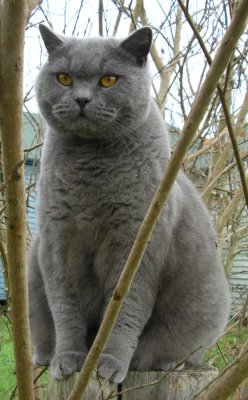
\includegraphics[width=2in]{images/cat.jpg}

\includegraphics[width=2in]{images/cat_tinted.jpg}
\end{figure}

\subsection{MATLAB文件}

%The functions scipy.io.loadmat and scipy.io.savemat allow you to read and write MATLAB files. You can read about them in the documentation.

函数 \lstinline|scipy.io.loadmat| 和 \lstinline|scipy.io.savemat| 允许你读写 MATLAB 函数。具体请查看\href{http://docs.scipy.org/doc/scipy/reference/io.html}{文档}。

\subsection{点之间的距离} %Distance between points

%SciPy defines some useful functions for computing distances between sets of points.

Scipy 定义了一些有用的函数,可计算集合中点之间的距离。

%The function scipy.spatial.distance.pdist computes the distance between all pairs of points in a given set:

函数 \lstinline|scipy.spatial.distance.pdist| 计算给定集合中所有两点之间的距离:
\lstinputlisting[]{code/scipy_pdist.py}

具体细节请阅读\href{http://docs.scipy.org/doc/scipy/reference/generated/scipy.spatial.distance.pdist.html}{文档}。
%A similar function (scipy.spatial.distance.cdist) computes the distance between all pairs across two sets of points; you can read about it in the documentation.

函数 \lstinline|scipy.spatial.distance.cdist| 可以计算不同集合中点的距离。

